\graphicspath{{3cyclic/asy/}}

\section{Cyclic \& Finite Abelian Groups}\label{chap:cyclic}

In this chapter we consider a general family of groups and see how to combine these to describe any finite abelian group.

\subsection{Definitions and Basic Examples}\label{sec:cycdef}

The foundational idea of a cyclic group is that it may be generated from a single element.

\begin{examples}{}{cyclicexmotiv}
	\exstart The integers $(\Z,+)$ are generated by the element 1: all integers may be produced by repeatedly combining 1 using only the group operation ($+$) and inverses ($-$). For instance,
	  \[
	  	-4=-(1+1+1+1)
	  \]
	\begin{enumerate}\setcounter{enumi}{1}
	  \item\label{ex:cyclicexmotiv2} The modular arithmetic groups $(\Z_n,+_n)$ (Section \ref{sec:modarith}) are also generated by (the remainder) 1. Since the group is finite, inverses are not necessary. For instance,
	  \[
	  	\Z_4=\{0,1,2,3\}=\{0,\ 1,\ 1+1,\ 1+1+1\}
	  \]
	 	\item The group $R_n$ of rotations of a regular $n$-gon (Definition \ref{defn:rot-dihedral}) is generated by the `1-step' rotation $\rho_1$: that is, $\rho_k=\rho_1^k$.
	\end{enumerate}
\end{examples}

We formalize this idea by considering the subset of a group that may be produced from a single element, the group operation, and inverses.

\begin{lemm}{Cyclic subgroup}{cyclicdef}
	Let $G$ be a group and $g\in G$. The set
	\[
		\ip{g}:=\{g^n:n\in\Z\}=\{\ldots,g^{-1},e,g,g^2,\ldots\}
	\]
	is a subgroup of $G$. We call this the \emph{cyclic subgroup\footnotemark{} generated by $g$.}
\end{lemm}

\footnotetext{%
	Since this is an abstract result, the lemma is written multiplicatively. If $G$ is an additive group, then cyclic subgroups are written $\ip{g}=\{ng:n\in\Z\}=\{\ldots,-2g,-g,0,g,2g,3g,\ldots\}$. As in Example \ref*{ex:cyclicexmotiv}.\ref{ex:cyclicexmotiv2}, for finite cyclic groups convention dictates that the identity element is written first, e.g.{} $\ip{g}=\{e,g,g^2,\ldots,g^{n-1}\}$. %
}

\begin{proof}
	We follow the subgroup criterion (Theorem \ref{thm:subgroup}).
	\begin{quote}
		\begin{description}
			\item[\emph{Non-emptiness}:] Plainly $g\in\ip g$.
			\item[\emph{Closure}:] Every element of $\ip g$ has the form $g^k$ for some $k\in \Z$. The required condition follows from standard exponential notation (Definition \ref{defn:assoc}): $g^k\cdot g^l=g^{k+l}\in\ip g$.
			\item[\emph{Inverses}:] This is Exercise \ref*{sec:groupaxioms}.\ref{exs:multinverse2}: $(g^k)^{-1}=g^{-k}\in\ip g$.
		\end{description}
	\end{quote}
	\vspace{-18pt}
\end{proof}

\begin{defn}{Cyclic group}{cyclic}
	A group $G$ is \emph{cyclic} if it has a \emph{generator}: $\exists g\in G$ such that $G=\ip g$.\smallbreak
	In any group $G$, the \emph{order of an element $g$} is the order (cardinality) of the cyclic subgroup $\ip g\le G$.
\end{defn}

\textcolor{red}{Warning!} Don't confuse the \emph{order of a group} $G$ with the \emph{order of an element} $g\in G$. Cyclic groups are precisely those containing elements (generators) whose order equals that of the group!


\goodbreak


\begin{examples*}{\ref{ex:cyclicexmotiv} cont}{}
	\exstart $\Z=\ip{1}=\ip{-1}$ is generated by either 1 or $-1$. The cyclic subgroup generated by 2 is the group of even numbers under addition
	\[
		\ip 2=\{\ldots,-2,0,2,4,\ldots\}=\{2m:m\in\Z\}=2\Z
	\]
	\begin{enumerate}\setcounter{enumi}{1}
	  \item $\Z_n$ is generated by both 1 and $-1=n-1$, but may have other generators (we'll consider how to find them all shortly). For instance, $\Z_5$ is generated also by 2:
	  \[
	  	\ip 2=\{0, 2,\ 2+2,\ 2+2+2,\ \ldots\}=\{0, 2, 4, 1, 3\} =\Z_5
	  \]
		\item $R_n=\ip{\rho_1}=\{e,\rho_1,\rho_1^2,\ldots,\rho_1^{n-1}\}$. As with $\Z_n$, this group typically has other generators.
	\end{enumerate}
\end{examples*}


Another commonly encountered family of cyclic groups arise as subgroups of $(\C^\times,\cdot)$ (or $(S^1,\cdot)$).

\begin{defn}{Roots of Unity}{}
	Let $n\in\N$. The group of \emph{$n\th$ roots of unity} $U_n$ is the cyclic subgroup of $(S^1,\cdot)$ generated by $\zeta:=e^{\frac{2\pi i}n}$:
	\[
		U_n:=\ip{\zeta}=\bigl\{1,\zeta,\zeta^2,\cdots,\zeta^{n-1}\bigr\}
	\]
	These are precisely the $n$ complex solutions to the equation $z^n=1$. To emphasize $n$, write $\zeta_n=\smash[t]{e^{\frac{2\pi i}n}}$. 
\end{defn}

\begin{minipage}[t]{0.75\linewidth}\vspace{-5pt}
	For instance $U_2=\ip{-1}=\{1,-1\}$ and $U_4=\ip{i}=\{1,i,-1,-i\}$. In general, the $n\th$ roots are the vertices of a regular $n$-gon centered at 0 with radius 1:
	\[
		\nm{\zeta^k}=\nm\zeta^k=1
		\quad\text{and}\quad
		\arg\zeta^k=\arg e^{\frac{2\pi k}{n}}=\tfrac{2\pi k}n=k\arg\zeta
	\]
	We stop listing the elements at $\zeta^{n-1}$ since $\zeta^n=e^{2\pi i}=1$. The periodicity of the complex exponential $(e^{i\theta}=1\Longleftrightarrow \theta\in 2\pi\Z)$ results in a simple tie-in with modular arithmetic:
	\[
		\zeta^k=\zeta^l\iff 1=\zeta^{k-l}=e^{\frac{2\pi i(k-l)}n}\iff k\equiv l\pmod n
	\]
\end{minipage}
\hfill
\begin{minipage}[t]{0.24\linewidth}\vspace{-5pt}
	\centering
	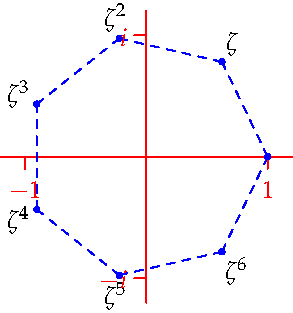
\includegraphics[scale=0.8]{cyclic-rootunity}\\
	Seventh roots: $\zeta_7=e^{\frac{2\pi i}7}$
\end{minipage}
\bigbreak



\begin{examples}{}{unisoex}
	\exstart Observe that $\zeta_6^2=(e^{\frac{2\pi i}6})^2 =e^{\frac{2\pi i}3} =\zeta_3$.\par
	\begin{enumerate}\setcounter{enumi}{1}
		\begin{minipage}[t]{0.75\linewidth}\vspace{-8pt}
			\item[]This produces a subgroup relationship: writing $\textcolor{blue}{\zeta}=\zeta_6$, we have
			\[
				U_3 = \bigl\{\textcolor{red}{1},\textcolor{red}{\zeta^2},\textcolor{red}{\zeta^4}\bigr\}  < U_6 = \bigl\{\textcolor{red}{1},\textcolor{blue}{\zeta},\textcolor{red}{\zeta^2},\zeta^3,\textcolor{red}{\zeta^4},\zeta^5\bigr\}
			\]
			The picture makes this geometrically trivial (compare Example \ref*{ex:hexsubgroup}.\ref{ex:hexsubgroup2}).
		\end{minipage}
		\hfill
		\begin{minipage}[t]{0.24\linewidth}\vspace{-32pt}
			\flushright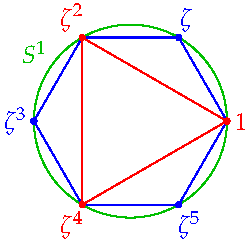
\includegraphics[scale=0.8]{cyclic-hexagon}
		\end{minipage}
	  
	  
	  \item\label{ex:unisoex2} (Example \ref{ex:z3r3iso}, cont.) \ Below is the Cayley table for $U_3$. Writing $1=\zeta^0$ and $\zeta=\zeta^1$ makes the isomorphic relationship with $(\Z_3,+_3)$ and $(R_3,\circ)$ obvious: $(U_3,\cdot)\cong (\Z_3,+_3)\cong (R_3,\circ)$.
		\[
			\def\arraystretch{1.1}
			\begin{array}{c||c|c|c}
				\cdot&1&\zeta&\zeta^2\\\hline\hline
				1&1&\zeta&\zeta^2\\\hline
				\zeta&\zeta&\zeta^2&1\\\hline
				\zeta^2&\zeta^2&1&\zeta
			\end{array}
			\qquad
			\begin{array}{c||c|c|c}
				\cdot&\zeta^{\textcolor{red}{0}}&\zeta^{\textcolor{blue}{1}}&\zeta^{\textcolor{Green}{2}}\\\hline\hline
				\zeta^{\textcolor{red}{0}}&\zeta^{\textcolor{red}{0}}&\zeta^{\textcolor{blue}{1}}&\zeta^{\textcolor{Green}{2}}\\\hline
				\zeta^{\textcolor{blue}{1}}&\zeta^{\textcolor{blue}{1}}&\zeta^{\textcolor{Green}{2}}&\zeta^{\textcolor{red}{0}}\\\hline
				\zeta^{\textcolor{Green}{2}}&\zeta^{\textcolor{Green}{2}}&\zeta^{\textcolor{red}{0}}&\zeta^{\textcolor{blue}{1}}
			\end{array}
			\qquad
			\begin{array}{c||c|c|c}
				+_3&\textcolor{red}{0}&\textcolor{blue}{1}&\textcolor{Green}{2}\\\hline\hline
				\textcolor{red}{0}&\textcolor{red}{0}&\textcolor{blue}{1}&\textcolor{Green}{2}\\\hline
				\textcolor{blue}{1}&\textcolor{blue}{1}&\textcolor{Green}{2}&\textcolor{red}{0}\\\hline
				\textcolor{Green}{2}&\textcolor{Green}{2}&\textcolor{red}{0}&\textcolor{blue}{1}
			\end{array}
			\qquad
			\begin{array}{c||c|c|c}
				\circ&\rho_{\textcolor{red}{0}}&\rho_{\textcolor{blue}{1}}&\rho_{\textcolor{Green}{2}}\\\hline\hline
				\rho_{\textcolor{red}{0}}&\rho_{\textcolor{red}{0}}&\rho_{\textcolor{blue}{1}}&\rho_{\textcolor{Green}{2}}\\\hline
				\rho_{\textcolor{blue}{1}}&\rho_{\textcolor{blue}{1}}&\rho_{\textcolor{Green}{2}}&\rho_{\textcolor{red}{0}}\\\hline
				\rho_{\textcolor{Green}{2}}&\rho_{\textcolor{Green}{2}}&\rho_{\textcolor{red}{0}}&\rho_{\textcolor{blue}{1}}
			\end{array}
		\]
		
		\goodbreak
		
		For a little practice here is a formal argument that $\Z_3\cong U_3$: we show explicitly that 
		\[
			\mu:\Z_3\to U_3:x\mapsto\zeta^x
		\]
		is an isomorphism. Since the domain $\Z_3$ consists of \emph{equivalence classes}, this requires a little care.
	\begin{description}
  	\item[\emph{Well-definition}:] We must prove that if $x=y$ in $\Z_3$, then $\mu(x)=\mu(y)$.\par
  	Given $x=y\in\Z_3$, then (\emph{as integers}) $x=y+3k$ for some integer $k$. But then
  	\[
  		\mu(x) =\zeta^x =\zeta^{x+3k} =\zeta^y(\zeta^{3})^k =\zeta^y =\mu(y)
  	\]
  	\item[\emph{Homomorphism}:] $\mu(x+y) =\zeta^{x+y} =\zeta^x\zeta^y =\mu(x)\mu(y)$
  	\item[\emph{Injectivity}:] $\mu(x)=\mu(y)\Longrightarrow \zeta^x=\zeta^y\Longrightarrow \zeta^{x-y}=1\Longrightarrow x\equiv y\pmod 3\Longrightarrow x=y$ in $\Z_3$.\par
  	(Notice how injectivity is the converse of well-definition!)
  	\item[\emph{Surjectivity}:] $\operatorname{range}\mu =\{\zeta^x:x\in\Z\} =\{1,\zeta,\zeta^2\} =U_3$, since $\zeta^{x+3k}=\zeta^x$.
	\end{description}
In the next section we'll essentially repeat this discussion in the abstract, so make sure this example makes sense before moving on.
	\end{enumerate}
\end{examples}



\begin{exercises}
	Key concepts:\quad \emph{Generator\quad Order of an element\quad Cyclic (sub)group\quad Roots of unity}
	
	\begin{enumerate}	  
	  \item Compute the cyclic subgroup $\ip{12}$ of $\Z_{20}$ (write the elements in the order generated).
	  
	  
		\item Find/describe \emph{all} the generators of each cyclic group.
	  \begin{enumerate}
	      \item \makebox[120pt][l]{$(\Z,+)$ \hfill (b) }
	      $\{2^n3^{-n}:n\in\Z\}$ under multiplication
	      \setcounter{enumii}{2}
	      \item \makebox[120pt][l]{$(\Z_5,+_5)$ \hfill (d) }
	      $\left\{\begin{smatrix} a&0\\0&a \end{smatrix},\begin{smatrix} 0&b\\-b&0 \end{smatrix}: a,b=\pm 1\right\}$ under multiplication
	  \end{enumerate}
	  
	  
	  \item State all cyclic subgroups of $\Z_{9}$. What is the order of each element?
	
	
	  \item Recall Example \ref{ex:d3}. What is the cyclic subgroup of $D_3$ generated by $\rho_1$? Generated by $\mu_1$?
	  
	  
	  \item\label{exs:kleinnoncyclic}\begin{enumerate}
	    \item Find all cyclic subgroups of the Klein four-group $V$. What is the order of each element?
			\item $V$ is a \emph{finite} non-cyclic group. Give an example of an \emph{infinite} non-cyclic group, and explain how you know you are correct.
	  \end{enumerate}
	  
	  
	  \item Compute the cyclic subgroup $\ip{\zeta_8^5}$ of $U_8$, listing its elements in the order generated. 
	  	  
	  
		\item\begin{enumerate}
		  \item Prove that $(U_3,\cdot)$ is a subgroup of $(U_9,\cdot)$.
		  \item Complete the sentence and prove your assertion:
		  \begin{quote}
		  	$U_m\le U_n$ if and only if \underline{\qquad\scriptsize(relationship between $m$ and $n$)\qquad}
		  \end{quote}
		\end{enumerate}
	    	
		  
	  \item\label{exs:z5times2}
	  \begin{enumerate}
	    \item Show that $\Z_5^\times=\{1,2,3,4\}$ forms a cyclic group under \emph{multiplication} modulo 5.
	  	\item What about $\Z_8^\times=\{1,3,5,7\}$ under multiplication modulo 8? To what well-known group is this isomorphic?
	  \end{enumerate}
	  
	  
	  \item Suppose that a cyclic group $G$ has order $\nm G\ge 3$. Explain why it has \emph{at least two} generators.
	
		
		\item Modeling Example \ref*{ex:unisoex}.\ref{ex:unisoex2}, prove explicitly that $\Z_n\cong U_n$ for any $n\in\N$.
		
	  
	  \item In contrast to the real case (Example \ref*{ex:expiso}.\ref{ex:expiso1}), verify that $\phi:\C\to\C^\times:z\mapsto e^z$ is a homomorphism $(\C,+)\cong(\C^\times,\cdot)$ but \emph{not} an isomorphism.
	 
	\end{enumerate}
\end{exercises}

\clearpage



\subsection{The Classification and Structure of Cyclic Groups}\label{sec:cyclicclass}

This section is significantly more abstract that what has come before: take your time, read carefully, and use the examples to help. Our goal is to describe general properties of all cyclic groups, including  their generators and subgroup structures. The first result is, mercifully, very simple.

\begin{lemm}{}{}
	Every cyclic group is abelian.
\end{lemm}

\begin{proof}
	Let $G=\ip g$. Any two elements of $G$ can be written $g^k,g^l$ for some $k,l\in\Z$. The result follows from standard exponential notation and the fact that addition of integers is commutative:
	\[
		g^kg^l=g^{k+l}=g^{l+k}=g^lg^k\tag*{\qedhere}
	\]
\end{proof}

Note that the converse is \emph{false}: the Klein four-group $V$ is abelian but not cyclic (Exercise \ref*{sec:cycdef}.\ref{exs:kleinnoncyclic}).\medbreak

Our major classification theorem proves a pattern you've likely already guessed.

\begin{thm}{Isomorphs}{cyclicisomorph}
	Every cyclic group $G=\ip g$ is isomorphic either to $\Z$ or to some $\Z_n$:
	\begin{itemize}
	  \item If $G$ is infinite, then $G\cong\Z$.
	  \item If $G$ is finite with order $n$, then $G\cong\Z_n$.
	\end{itemize}
	In either case, $\mu:\Z_{(n)}\to G:x\mapsto g^x$ is an explicit isomorphism.
\end{thm}

To help understand the theorem and set up the proof, some remarks and examples are helpful.
\begin{description}
  \item[Map Generator to Generator] The isomorphism maps the generator $1\in\Z_{(n)}$ to the generator $g$ of $G$. Together with the homomorphism property, this idea \emph{defines} $\mu$
  \[
  	\mu(1)=g\implies \mu(x)=\mu(x+\cdots +x)=\bigl(\mu(1)\bigr)^x=g^x
  \]
  This observation makes it easy to find suitable isomorphisms in examples.
  \item[\emph{The} Cyclic Group of Order $n$?] The theorem says that, \emph{up to isomorphism}, there is a unique cyclic group of order $n$. For this reason, many algebraists use the symbol $\Z_n$ (or $C_n$ for `cyclic') to refer to any example of a cyclic group of order $n$ (e.g. $R_n$, $U_n$, etc.). For clarity, in these notes, $\Z_n$ will always be the explicit group of remainders under addition modulo $n$.
  \item[The Order of $G=\ip g$] It is helpful to introduce a set of positive integers
  \[
  	S:=\{m\in\N:g^m=e\} \tag{$mg=e$ if $G$ is additive}
  \]
  This set plays a crucial role in the proof, distinguishing the finite/infinite cases and detecting the order of $G$\ldots
\end{description}


\begin{examples}{}{}
	\exstart $\Z_4=\ip 1$ is additive, so $S=\{m\in\N:m=0\in\Z_4\}=\{\textcolor{red}{4},8,12,\ldots\}$. The minimal element $\textcolor{red}{4}$ is plainly the order of $\nm{\Z_4}$.
	\begin{enumerate}\setcounter{enumi}{1}%\itemsep2pt
	  \item (Example \ref*{ex:unisoex}.\ref{ex:unisoex2}) \ In $U_3=\ip\zeta$, we have $\zeta^m=1\Longleftrightarrow 3\mid m$, whence $S=\{\textcolor{red}{3},6,9,\ldots\}$. Plainly $\textcolor{red}{3}$ is the order of $U_3$. Moreover $\mu(x)=\zeta^x$ is the isomorphism $\mu:\Z_3\to U_3$ seen previously!
	  
	  \goodbreak
	  
	  \item $5\Z=\ip 5$ is an infinite cyclic group. In this case, $S=\{m\in\N:5m=0\}=\emptyset$ is \emph{empty}. We have an isomorphism $\mu:\Z\to 5\Z:x\mapsto 5x$ \ (map the generator 1 of $\Z$ to the generator 5 of $5\Z$).
	\end{enumerate}
\end{examples}




\begin{proof}
	We first establish that $\mu$ is a bijection. The generic cases depend on the minimal element of $S$.
	\begin{description}\itemsep2pt
		\item[Case 1: $S=\emptyset$.]\quad Suppose $x>y$ and that $g^x=g^y$. Then $g^{x-y}=e\Longrightarrow x-y\in S$: contradiction. The elements $\ldots,g^{-2},g^{-1},e,g,g^2,\ldots$ are \emph{distinct,} and so $\mu:\Z\to G:x\mapsto g^x$ is bijective.
		\item[Case 2: $\min S=n$.]\quad We first check that $\mu:\Z_n\to G:x\mapsto g^x$ is well-defined:
		\begin{align*}
			y=x\in\Z_n&\implies y=x+kn\text{ for some $k\in\Z$ \ (as integers)}\\
			&\implies \mu(y) =g^y =\textcolor{red}{g^{x+kn}=g^x(g^n)^k =g^x} =\mu(x) \tag{$n\in S$, so $g^n=e$}
		\end{align*}
		This \textcolor{red}{moreover} tells us that $G$ is \emph{finite} (there are at most $n$ distinct elements of $G$)
		\[
			G=\ip{g} =\{\ldots,g^{-2},g^{-1},e,g,g^2,\ldots\} =\{e,g,\ldots,g^{n-1}\}
		\]
		Now suppose two of these terms were equal; if $0\le y\le x\le n-1$, then
		\[
			g^x=g^y\implies g^{x-y}=e\implies x=y \tag{$0\le x-y\le n-1<n=\min S$}
		\]
		We conclude that $G=\{e,g,\ldots,g^{n-1}\}$ has order $n$, and that $\mu$ is a bijection.
	\end{description}\medskip
	Finally, note that the homomorphism property in both cases is merely standard exponential notation
	\[
		\mu(x+y)=g^{x+y}=g^xg^y=\mu(x)\mu(y)\tag*{\qedhere}
	\]
\end{proof}

As advertised, the use of $S$ in the proof yields a useful alternative notion for the order of an element.

\begin{cor}{Order of an element}{orderdefn}
	If finite, the order of $g$ equals the minimal positive integer $n$ for which $g^n=e$. Moreover $g^m=e\Longleftrightarrow n\mid m$.
\end{cor}

Otherwise said, if $g$ has order $n$, then $S=\{m\in\N:g^m=e\}=\{kn:k\in\N\}$ is the set of positive multiples of $n$.



\begin{examples}{}{}
	\exstart The group of $7\th$ roots of unity $U_7$ is isomorphic to $\Z_7$ via $\mu:\Z_7\to U_7:k\mapsto \zeta_7^k$. As a sanity check, observe that $7=\min\{m\in\N:\zeta_7^m=1\}$ is indeed the order of $\zeta_7 =e^{\frac{2\pi i}7}$.
	\begin{enumerate}\setcounter{enumi}{1}
		\item $(\R,+)$ is non-cyclic since its (uncountable) cardinality is larger than that of the integers. This is also straightforward directly: if $\R=\ip x$ were cyclic ($x\neq 0$), then we obtain the contradiction
		\[
			\frac x2\notin\{\ldots,-2x,-x,0,x,2x,3x\ldots\}=\ip x=\R\ni\frac x2
		\]
		The same argument shows that, for instance, that $(\Q,+)$ is non-cyclic.
		
		\item Let $\xi=\smash[t]{e^{\frac{2\pi i}{\sqrt 2}}}$ and consider the cyclic subgroup $G:=\ip\xi<(\C^\times,\cdot)$. For integers $m$, observe that
		\[
			\xi^m=e^{\frac{2\pi im}{\sqrt 2}}=1\iff \tfrac m{\sqrt 2}\in\Z\iff m=0
		\]
		We conclude that $G$ is an \emph{infinite} cyclic group and that $\mu:\Z\to G:z\mapsto\xi^z$ is an isomorphism. Multiplication by $\xi$ essentially performs an irrational fraction $(\frac 1{\sqrt 2})$ of a full rotation.
	\end{enumerate}
\end{examples}


\goodbreak


\boldsubsubsection{Subgroups of Cyclic Groups are also Cyclic!}

For the remainder of this section we describe the complete subgroup structure of all cyclic groups. Our approach is motivated by a simple example.

\begin{example}{}{}
	The cyclic subgroup $2\Z\le\Z$ is generated by 2: the \emph{minimal positive integer} in the subgroup.
\end{example}

For an abstract subgroup $H$ of a cyclic group $G=\ip g$, our goal is to identify a suitable `minimal element' of $H$ and then demonstrate that this generates $H$.

\begin{thm}{Subgroups of Cyclic Groups}{cyclic1}
	Every subgroup of a cyclic group is cyclic.
\end{thm}

\begin{proof}
	Suppose $H$ is a subgroup of $G=\ip g$. Let $s$ be the smallest \emph{positive} integer\footnotemark{} such that $g^s\in H$.
	We prove that $H$ is generated by $g^s$ by establishing the set equality $H=\ip{g^s}$.
	\begin{description}\itemsep0pt
		\item[$(\supseteq)$] Since $H$ is a group, the closure and inverse axioms force $(g^s)^k\in H$ for all $k\in\Z$.
		\item[$(\subseteq)$] Let $g^m\in H$. We must prove that $g^m\in\ip{g^s}$. By the division algorithm, there exist unique integers $q,r$ such that
		\[
			m=qs+r\quad\text{and}\quad 0\le r<s
		\]
		Since $H$ satisfies the closure and inverse axioms,
		\[
			g^m=g^{qs+r}=(g^s)^qg^r\implies g^r=(g^s)^{-q}g^m\in H \tag{$\ast$}
		\]
		The minimality of $s$ forces $r=0$, from which we conclude that $g^m=(g^s)^q\in\ip{g^s}$.\qedhere 
	\end{description}
\end{proof}


\footnotetext{%
	 This exists for two reasons:
	\begin{enumerate}
	  \item $H$ is a non-empty subset of $G=\ip g$ and so must contain some element $g^k$. We may assume $k\ge 1$ since the subgroup also contains $g^{-k}$ (inverse axiom).
	  \item The set of natural numbers $\{k\in\N:g^k\in H\}$ is non-empty and so (well-ordering) has a minimal element $s$.
	\end{enumerate}
	Note that $s=1\Longleftrightarrow H=\ip{e}$ is the trivial subgroup ($g^1=e^1=e\in H$). In this special case the division algorithm argument is trivial: every $m=q\cdot 1+0$ is immediately a multiple of 1, and $g^m=e$ for all $m$. 
}

If the proof seems hard, try rewriting it for our motivational example, where $G=\Z$, $H=2\Z$ and $s=2$; remember that $G$ is \emph{additive}, so ($\ast$) is simply $r=-2s+m\in 2\Z$!

\medskip

We finish by considering the finite and infinite cases separately. The latter is very simple.

\begin{cor}{Subgroups of infinite cyclic groups}{infcyclic}
	If $G$ is an infinite cyclic group and $H\le G$, then either $H=\{e\}$ is trivial, or $H\cong G$.
\end{cor}

The proof as an exercise---just generalize the following generic example!

\begin{example}{}{}
	We write things out explicitly in additive notation when $G=\Z$. By Theorem \ref{thm:cyclic1}, every subgroup has the form $\ip s=s\Z$ (the multiples of $s\in\Z$). There are two generic situations:
	\begin{itemize}
	  \item If $s=0$ we have the trivial subgroup: $\ip 0=\{0\}$.
	  \item If $s\neq 0$, then $s\Z$ is isomorphic to $\Z$ via the isomorphism $\mu:\Z\to s\Z:x\mapsto sx$.
	\end{itemize}
\end{example}


\goodbreak


\emph{Finite} cyclic groups are more complicated, so we first illustrate the main result with an example.

\begin{example}{}{u6z6explicit}
	Consider the 6\th{} roots of unity $U_6=\{1,\zeta,\zeta^2,\zeta^3,\zeta^4,\zeta^5\}$. Since every subgroup of $U_6$ is necessarily cyclic (Theorem \ref{thm:cyclic1}), it is enough to consider each cyclic subgroup $\ip z$ in turn (for each $z\in U_6$). We obtain three proper subgroups, as arranged in the subgroup diagram below.
	\[
		\makebox[230pt][l]{%
			$\def\arraystretch{1.05}
			\begin{array}[t]{l|c}
				z & \text{subgroup}\ip z\\ \hline
				1 & \{1 \} \\
				\textcolor{red}{\zeta} & \textcolor{red}{\{1,\zeta,\zeta^2,\zeta^3,\zeta^4,\zeta^5\}}\\
				\textcolor{blue}{\zeta^2} & \textcolor{blue}{\{1,\zeta^2,\zeta^4\}}\\
				\textcolor{Green}{\zeta^3} & \textcolor{Green}{\{1,\zeta^3\}}\\
				\textcolor{blue}{\zeta^4} & \textcolor{blue}{\{1,\zeta^4,\zeta^2\}}\\
				\textcolor{red}{\zeta^5} & \textcolor{red}{\{1,\zeta^5,\zeta^4,\zeta^3,\zeta^2,\zeta\}}
			\end{array}$
		}
		\makebox[0pt][c]{%
			$\xymatrix @C0pt @R24pt{%
				& \textcolor{red}{\ip{\zeta}}=U_6 \ar@{-}[dl] \ar@{-}[dr] & \\
				\textcolor{blue}{\ip{\zeta^2}}=U_3 \ar@{-}[dr] & & \textcolor{Green}{\ip{\zeta^3}}=U_2 \ar@{-}[dl] \\
				& \ip{1}=U_1 &
			}$
		}
	\]
	Observe the repetitions: $\ip{\textcolor{red}{\zeta}}=\ip{\textcolor{red}{\zeta^5}}=U_6$ and $\ip{\textcolor{blue}{\zeta^2}}=\ip{\textcolor{blue}{\zeta^4}}=U_3$. Note also that we really do have \emph{equality} of groups here: for instance, $\textcolor{blue}{\zeta^2}=(e^{\frac{2\pi i}6})^2=e^{\frac{2\pi i}3}$ is a generator of $U_3$.
	\medbreak
	For comparison, here is the same data for subgroups of the additive group $(\Z_6,+_6)$.
	\[
		\makebox[230pt][l]{%
			$\def\arraystretch{1.05}
			\begin{array}[t]{l|c}
				x & \text{subgroup}\ip x\\ \hline
				0 & \{0\} \\
				\textcolor{red}{1} & \textcolor{red}{\{0,1,2,3,4,5\}}\\
				\textcolor{blue}{2} & \textcolor{blue}{\{0,2,4\}}\\
				\textcolor{Green}{3} & \textcolor{Green}{\{0,3\}}\\
				\textcolor{blue}{4} & \textcolor{blue}{\{0,4,2\}}\\
				\textcolor{red}{5} & \textcolor{red}{\{0,5,4,3,2,1\}}
			\end{array}$
		}
	\makebox[0pt][c]{%
		$\xymatrix @C0pt @R24pt{%
			& \textcolor{red}{\ip{1}}=\Z_6 \ar@{-}[dl] \ar@{-}[dr] & \\
			\textcolor{blue}{\ip{2}}\cong\Z_3 \ar@{-}[dr] & & \textcolor{Green}{\ip{3}}\cong\Z_2 \ar@{-}[dl] \\
			& \ip{0}\cong\Z_1 &
			}$
		}
	\]
	Since $U_6\cong\Z_6$, differences are entirely notational. One subtle distinction is that we don't use \emph{equals} in the second subgroup diagram: for instance, $\textcolor{blue}{\ip{2}}=\{0,2,4\}$ is \emph{isomorphic} but \emph{not equal} to $\Z_3=\{0,1,2\}$.
\end{example}

The Example should suggest a pattern (previewed in Lemma \ref{lemm:cyclicsg}): the subgroups of $\Z_n$ are precisely those generated by the divisors of $n$, with one subgroup for each divisor: 
\[
	\tcbhighmath{d\mid n\Longrightarrow \ip d\cong\Z_{\frac nd},\quad\text{moreover }\gcd(s,n)=d\Longrightarrow \ip s=\ip d}
\]
Our final result merely asserts this for general finite cyclic groups.


\begin{cor}{Subgroups of finite cyclic groups}{subscyclic}
	Let $G=\ip g$ have order $n$. For each divisor of $n$, $G$ has a \textbf{unique subgroup} with this order; these are moreover the \textbf{only} subgroups of $G$.\par
	More precisely, 
	\[
		d=\gcd(s,n)\Longrightarrow \ip{g^s}=\langle{g^d}\rangle, \quad\text{where this subgroup has order $\tfrac nd$ \ (isomorphic to $\Z_{\frac nd}$)}
	\]
	In particular: $g^s$ has order $\frac n{\gcd(s,n)}$ and generates $G$ if and only if $\gcd(s,n)=1$.
\end{cor}

As with Theorem \ref{thm:cyclic1}, if the proof seems hard, try rewriting it when $G=\Z_n$.

\begin{proof}
	Suppose $d=\gcd(s,n)$. We prove set inclusion in both directions.
	\begin{description}
		\item[$(\subseteq)$] Since $d$ divides $s$, we have $s=kd$ for some $k\in\Z$. But then
		\[
			g^s=(g^d)^{k}\in\bigl\langle g^d\big\rangle \implies (g^s)^t=(g^d)^{kt}\implies  \ip{g^s}\subseteq\bigl\langle g^d\big\rangle
		\]
		\item[$(\supseteq)$] Apply Bézout's identity (extended Euclidean alg.): $d=\kappa s+\lambda n$ for some $\kappa,\lambda\in\Z$, whence
		\[
			g^d=(g^s)^\kappa (g^n)^\lambda=(g^s)^\kappa\in\ip{g^s} \implies \bigl\langle g^d\big\rangle\subseteq\ip{g^s}
		\]
	\end{description}
	To finish, note that since $d\mid n$, there are precisely $\frac nd$ elements of $\ip{g^d}$:
	\[
		\langle{g^d}\rangle=\bigl\{e,g^d,g^{2d},\ldots,g^{n-d}\bigr\}\tag*{\qedhere}
	\]
\end{proof}


\begin{example}{}{}
	\exstart $\Z_8$ is generated by $1,3,5$ and $7$: precisely the elements for which $\gcd(s,8)=1$. For example,
	\begin{enumerate}
  	\begin{minipage}[t]{0.87\linewidth}\vspace{-16pt}
		  \item[]
		  \[
		  	\ip 5=\{5,2,7,4,1,6,3,0\} =\Z_8
		  \]
		  Similarly, the subgroup $\ip 6=\{6,4,2,0\}$ has order $4=\frac 8{\gcd(6,8)}$. The complete collection of subgroups is in the table: the first column lists each divisor $d$ of 8 (the possible values of $\gcd(\textcolor{red}{x},8)$), while the second column has the explicit subgroup generated by each $\textcolor{red}{x}$, and the group isomorph $\Z_{\frac 8d}$. The `smallest' generator is used for each subgroup in the subgroup diagram. 
		  \[
		  	\def\arraystretch{1.05}
		    \begin{array}{c|l@{\,}l}
		    	d=\gcd(\textcolor{red}{x},8) & \multicolumn{2}{c}{\text{Subgroup } \ip{\textcolor{red}{x}}\cong\Z_{\frac 8d}}\\\hline
					1 & \{0, \textcolor{red}{1}, 2, \textcolor{red}{3}, 4, \textcolor{red}{5}, 6,  \textcolor{red}{7}\} &=\Z_8\\
					2 & \{0, \textcolor{red}{2}, 4, \textcolor{red}{6}\} &\cong\Z_4\\
					4 & \{0, \textcolor{red}{4}\} &\cong\Z_2\\
					8 & \{\textcolor{red}{0}\} &\cong\Z_1
		    \end{array}
		  \]
  	\end{minipage}
  	\hfill
  	\begin{minipage}[t]{0.1\linewidth}\vspace{35pt}
 			\flushright
	 		$\xymatrix{%
	 			\ip 1=\Z_{8} \ar@{-}[d]\\
				\ip 2\cong\Z_4 \ar@{-}[d]\\
				\ip 4\cong\Z_2 \ar@{-}[d]\\
				\ip 0\cong\Z_1
			}
			\hspace{-4pt}$
		\end{minipage}
		\setcounter{enumi}{1}
		\item	We repeat the discussion for $\Z_{30}$.
	  \[
	  	\def\arraystretch{1.05}
	  	\begin{array}[t]{c|l@{\,}l}
				d=\gcd(\textcolor{red}{x},30) & \multicolumn{2}{c}{\text{Subgroup } \ip{\textcolor{red}{x}}\cong\Z_{\frac{30}d}} \\\hline
				1 & \{0,\textcolor{red}{1},2,3,\ldots,\textcolor{red}{7},\ldots,\textcolor{red}{11},12,\textcolor{red}{13},\makebox[0cm][l]{$\ldots$} \hfill\\
				& \hfill\textcolor{red}{17},18,\textcolor{red}{19},\ldots,\textcolor{red}{23},\ldots,\textcolor{red}{29}\} &=\Z_{30}\\
				2 & \{0,\textcolor{red}{2},\textcolor{red}{4},6,\textcolor{red}{8},10,12,\textcolor{red}{14},\textcolor{red}{16},\hfill\\
				& \hfill 18,20,\textcolor{red}{22},24,\textcolor{red}{26},\textcolor{red}{28}\} &\cong\Z_{15}\\
				3 & \{0,\textcolor{red}{3},6,\textcolor{red}{9},12,15,18,\textcolor{red}{21},24,\textcolor{red}{27}\}  &\cong\Z_{10}\\
				5 & \{0,\textcolor{red}{5},10,15,20,\textcolor{red}{25}\} &\cong\Z_{6}\\
				6 & \{0,\textcolor{red}{6},\textcolor{red}{12},\textcolor{red}{18},\textcolor{red}{24}\}  &\cong\Z_{5}\\
				10 & \{0,\textcolor{red}{10},\textcolor{red}{20}\} &\cong\Z_{3}\\
				15 & \{0,\textcolor{red}{15}\} &\cong\Z_{2}\\
				30 & \{\textcolor{red}{0}\} &\cong\Z_{1}
	   \end{array}
	   \hfill
	   \xymatrix @C0pt @R30pt{%
			 	& \ip{1}=\Z_{30} \ar@{-}[dl] \ar@{-}[d] \ar@{-}[dr] & \\
				\ip{2}\cong \Z_{15} \ar@{-}[d] \ar@{-}[dr] & \ip{3}\cong\Z_{10} \ar@{-}[dl] \ar@{-}[dr] & \ip{5}\cong\Z_6 \ar@{-}[d] \ar@{-}[dl] \\
				\ip{6}\cong\Z_5 \ar@{-}[dr] & \ip{10}\cong \Z_{3} \ar@{-}[d] & \ip{15}\cong\Z_2 \ar@{-}[dl] \\
	 & \ip{0}\cong\Z_1 &
	 		}
	 		\hspace{-4pt}
	  \]
  \end{enumerate}
  
  You should consider how the \emph{shape} of the subgroup diagram for $\Z_n$ depends on the \emph{prime decomposition} of $n$: for instance, each prime appears exactly once in $30=2\cdot 3\cdot 5$.
\end{example}


\goodbreak


\begin{exercises}
	Key concepts:\quad \emph{Every cyclic group is isomorphic to $\Z$ or $\Z_n$ \qquad$g^m=e\iff (\operatorname{ord}g)\mid m$}
	\begin{quote}
		\emph{$\ip g\cong\Z_n\Longrightarrow \ip{g^s}\cong\Z_{\frac n{\gcd(s,n)}}$\qquad Subgroup diagrams for finite cyclic groups}
	\end{quote}
	
	
	\begin{enumerate}
		\item Construct the subgroup diagram and give a generator of each subgroup:
		\begin{enumerate}
		  \item $(\Z_{10},+_{10})$\qquad\qquad (b)\lstsp $(\Z_{42},+_{42})$.
		\end{enumerate}
	  
	  
	  \item A generator of the cyclic group $U_n$ group is known as a \emph{primitive $n\th$ root of unity.} For instance, the primitive 4\th\ roots are $\pm i$. Find all the primitive roots when:
	  \begin{enumerate}
	    \item $n=5$\hfill (b)\lstsp $n=6$\hfill (c)\lstsp $n=8$\hfill (d)\lstsp $n=15$\hspace*{\fill}\hspace*{\fill}
	  \end{enumerate}
		
		
		\item Find the complete subgroup diagram of $U_{p^2q}$ where $p,q$ are distinct primes.\par
		(\emph{Hint: Try $U_{12}$ first if this seems too difficult})
	  
	  
	  \item If $r\in\N$ and $p$ is prime, find all subgroups of $(\Z_{p^r},+_{p^r})$ and give a generator for each.
	  
	  		
	  \item\begin{enumerate}
	    \item Suppose $\mu:G\to H$ is an isomorphism of cyclic groups. If $g$ is a generator of $G$, prove that $\mu(g)$ is a generator of $H$. Do you really need $\mu$ to be an \emph{isomorphism} here?
	  
	  	\item If $G$ is an infinite cyclic group, how many generators has it got?
	  	
			\item Recall Exercise \ref*{sec:cycdef}.\ref{exs:z5times}. Describe an isomorphism $\phi:\Z_4\to\Z_5^\times$.
	  \end{enumerate} 
	  
	  
	  \item True or false: In \emph{any} group $G$, if $g$ has order $n$, then $g^s$ has order $\frac n{\gcd(s,n)}$. Explain.
	  
	  
	  \item Suppose $G=\ip g$ is infinite and $H=\ip{g^s}$ is an infinite subgroup. Prove Corollary \ref{cor:infcyclic} by describing an isomorphism $\mu:G\to H$.
	
	
	  \item Prove Corollary \ref{cor:orderdefn}: you'll need the division algorithm for the second part!
	  
	  
		\item Let $x,y$ be elements of a group $G$. If $xy$ has finite order $n$, prove that $yx$ also has order $n$.\par
		(\emph{Hint: $(xy)^m=x(yx)^{m-1}y$})
		
		
		\item For which real numbers $\theta$ is the multiplicative cyclic group $G=\ip{e^{2\pi i\theta}}\le\C^\times$ finite? Describe the order of $G$ in terms of $\theta$.
		

	%   \item Which of the following sets generate the group $(\Z_{30},+_{30})$? For those sets that do not generate the group give the subgroup that they do generate.
	%   \begin{enumerate}
	%       \item $\{2\}$
	%       \item $\{2,6\}$
	%       \item $\{2,3\}$
	%       \item $\{7\}$
	%       \item $\{12,18\}$
	%       \item $\{6,15\}$
	%   \end{enumerate}
		
		
		\item\label{exs:finitegen} Let $G$ be a group and $X$ a non-empty subset of $G$. The \emph{subgroup generated by $X$} is the subgroup created by making all possible combinations of elements and inverses of elements in $X$.
		\begin{enumerate}
		  \item Explain why $(\Z,+)$ is generated by the set $X=\{2,3\}$.
		  \item If $m,n\in(\Z,+)$, show $X=\{m,n\}$ generates $d\Z$, where $d=\gcd(m,n)$.
		  \item The Klein four-group $V$ is not cyclic, so it cannot be generated by a singleton set. Find a set of \emph{two} elements which generates $V$.
		  \item Describe the subgroup of $(\Q,+)$ generated by $X=\{\frac 12,\frac 13\}$.
		  \item (Hard) \ $(\Q,+)$ is plainly generated by the \emph{infinite} set $\{\frac 1n:n\in\N\}$. Explain why $(\Q,+)$ is \emph{not finitely generated}: i.e.\ there exists no \emph{finite} set $X$ generating $\Q$.\par
		  (\emph{Hint: Think about the prime factors of the denominators of elements of $X$})
		\end{enumerate}

	
	\end{enumerate}
\end{exercises}

\clearpage

\subsection{Direct Products \& Finite Abelian Groups}\label{sec:direct}


In this section we discuss a straightforward way to create new groups from old using the \emph{Cartesian product.} In the abstract, this discussion applies to any groups, though the ingredients in most of our examples will be cyclic.

\begin{example}{}{}
	Given $\Z_2=\{0,1\}$, the Cartesian product
	\[
		\Z_2\times \Z_2=\bigl\{(0,0),(0,1),(1,0),(1,1)\bigr\}
	\]
	has \emph{four} elements. This set inherits a binary structure via addition of co-ordinates
	\[
		(x,y)+(v,w):=(x+v,y+w)
	\]
	where $x+v$ and $y+w$ are both computed in $(\Z_2,+_2)$. This binary operation has an addition table that should looks very familiar: it has exactly the same structure as the Klein four-group!
	\begin{quote}
		\scalebox{1}{$%
			\begin{array}{c||c|c|c|c}
				+ & (0,0) & \textcolor{Green}{(0,1)} & \textcolor{red}{(1,0)} & \textcolor{blue}{(1,1)}\\\hline\hline
				(0,0) & (0,0) & \textcolor{Green}{(0,1)} & \textcolor{red}{(1,0)} & \textcolor{blue}{(1,1)}\\\hline
				\textcolor{Green}{(0,1)} & \textcolor{Green}{(0,1)} & (0,0) & \textcolor{blue}{(1,1)} & \textcolor{red}{(1,0)}\\\hline
				\textcolor{red}{(1,0)} & \textcolor{red}{(1,0)} & \textcolor{blue}{(1,1)} & (0,0) & \textcolor{Green}{(0,1)}\\\hline
				\textcolor{blue}{(1,1)} & \textcolor{blue}{(1,1)} & \textcolor{red}{(1,0)} & \textcolor{Green}{(0,1)} & (0,0)
			\end{array}%
		$}
		\qquad\scalebox{1.5}{$\leftrightsquigarrow$}\qquad
		\scalebox{1}{$%
			\begin{array}{c||c|c|c|c}
				\circ & e & \textcolor{Green}{a} & \textcolor{red}{b} & \textcolor{blue}{c}\\\hline\hline
				e & e & \textcolor{Green}{a} & \textcolor{red}{b} & \textcolor{blue}{c}\\\hline
				\textcolor{Green}{a} & \textcolor{Green}{a} & e & \textcolor{blue}{c} & \textcolor{red}{b}\\\hline
				\textcolor{red}{b} & \textcolor{red}{b} & \textcolor{blue}{c} & e & \textcolor{Green}{a}\\\hline
				\textcolor{blue}{c} & \textcolor{blue}{c} & \textcolor{red}{b} & \textcolor{Green}{a} & e
			\end{array}%
		$}
	\end{quote}
	We conclude that $\Z_2\times\Z_2\cong V$ is indeed a group.
\end{example}


This type of construction works in general.

\begin{thm}{Direct product}{directprod}
	The natural component-wise operation on the Cartesian product
	\[
		\smash[t]{\prod\limits_{k=1}^n} G_k=G_1\times\cdots\times G_n,\qquad (x_1,\ldots,x_n)\cdot(y_1,\ldots,y_n):=(x_1y_1,\ldots,x_ny_n)
	\]
	defines a group structure: the \emph{direct product.} This group is abelian if and only if each $G_k$ is abelian.
\end{thm}

The proof is a simple exercise. Being a Cartesian product, a direct product has order equal to the product of the orders of its components
\[
	\nm{\prod\limits_{k=1}^n G_k}=\prod\limits_{k=1}^n\nm{G_k}
\]
\vspace{2pt}


\begin{examples}{}{direct1}
	\exstart The direct product of the groups $(\Z_2,+_2)$ and $(\Z_3,+_3)$ is
	\[
		\Z_2\times\Z_3=\bigl\{(0,0),(0,1),(0,2),(1,0),(1,1),(1,2)\bigr\}
	\]
	This is abelian of order 6, so we might guess that it is isomorphic to $(\Z_6,+_6)$ and thus cyclic. This is indeed the case: simply observe that $(1,1)$ is a generator,
	\[
		\ip{(1,1)}=\bigl\{(0,0),(1,1),(0,2),(1,0),(0,1),(1,2)\bigr\}=\Z_2\times\Z_3
	\]
	In accordance with Theorem \ref{thm:cyclicisomorph}, $\mu(x)=(x,x)$ defines an isomorphism $\mu:\Z_6\cong\Z_2\times \Z_3$.

	\goodbreak

	\begin{enumerate}\setcounter{enumi}{1}
		\item If each $G_k$ is \emph{abelian} and \emph{written additively,} the direct product is sometimes called a \emph{direct sum},\footnotemark{}
		\[
			\bigoplus_{k=1}^nG_k=G_1\oplus\cdots\oplus G_n
		\]
		We won't use this notation, though you've likely encountered it in linear algebra: for instance, the direct sum of $n$ copies of the real line $\R$ is the familiar vector space
		\[
			\R^n=\bigoplus_{i=1}^n\R=\R\oplus\cdots\oplus\R
		\]
	\end{enumerate}
\end{examples}

\footnotetext{%
	In these notes a direct product/sum will only ever have \emph{finitely many} factors, in which case the concepts are identical. The slight difference in the concepts when there are infinitely many factors is not worth discussing here.%
}

\vspace{-5pt}


\boldsubsubsection{Orders of Elements in a Direct Product}

In Example \ref{ex:direct1}.1, we saw that the element $(1,1)\in\Z_2\times\Z_3$ had order 6 and thus generated the group. There is another general pattern here; to help spot it, consider another example.

\begin{example}{}{}
	We find the order of the element $(10,2)\in\Z_{12}\times \Z_8$? Recall Corollary \ref{cor:subscyclic}:
	\begin{itemize}\itemsep0pt
	  \item $10\in\Z_{12}$ has \textcolor{red}{order $6=\frac{12}{\gcd(10,12)}$}
	  \item $2\in\Z_8$ has \textcolor{blue}{order $4=\frac 8{\gcd(2,8)}$}
	\end{itemize}
	If we repeatedly add $(10,2)$ to itself, then the \textcolor{red}{first co-ordinate resets after 6} summations, whereas the \textcolor{blue}{second resets after 4}. For \emph{both} to reset simultaneously, we need a \emph{common multiple} of \textcolor{red}{6} and \textcolor{blue}{4} summands. We can check this explicitly:
	\[
		\bigl\langle(10,2)\bigr\rangle = \bigl\{(10,2), (8,4), (6,6), (4,\textcolor{blue}{0}), (2,2), (\textcolor{red}{0},4), (10,6), (8,\textcolor{blue}{0}), (6,2), (4,4), (2,6), (\textcolor{red}{0},\textcolor{blue}{0})\bigr\}
	\]
	The order of the element $(10,2)$ is indeed the \emph{least common multiple} $12=\lcm(6,4)$.
\end{example}


\begin{thm}{}{directorder}
	Suppose $x_k\in G_k$ has order $r_k$. Then $(x_1,\ldots,x_n)\in \prod\limits_{k=1}^n G_k$ has order $\lcm(r_1,\ldots,r_n)$.
\end{thm}

\begin{proof}
	We appeal to Corollary \ref{cor:orderdefn}:
	\[
		(x_1,\ldots,x_n)^m=(x_1^m,\ldots,x_n^m)=(e_1,e_2,\ldots,e_n)
		\iff \forall k,\ x_k^m=e_k 
		\iff \forall k,\ r_k\mid m
	\]
	The order is the minimal positive integer $m$ satisfying this, namely $m=\lcm(r_1,\ldots,r_n)$.
\end{proof}



\begin{example}{}{prodorder}
	Find the order of $(1,3,2,6)\in\Z_4\times\Z_7\times\Z_5\times\Z_{20}$.\smallbreak
	Again with reference to Corollary \ref{cor:subscyclic}, the element has order
	\[
		\lcm\left(\tfrac 4{\gcd(1,4)}, \tfrac 7{\gcd(3,7)}, \tfrac 5{\gcd(2,5)}, \tfrac{20}{\gcd(6,20)}\right) =\lcm(4,7,5,10)=140
	\]
\end{example}


\boldsubsubsection{When is a direct product of finite cyclic groups cyclic?}

Recall that $\Z_2\times\Z_3\cong \Z_6$ is cyclic, whereas $\Z_2\times\Z_2\cong V$ is non-cyclic. It is reasonable to hypothesize that the issue is whether the orders of the components are \emph{relatively prime.} 

\begin{cor}{}{prodprime}
	$\Z_m\times\Z_n$ is cyclic $\Longleftrightarrow \gcd(m,n)=1$. In such a case $\Z_m\times\Z_n\cong\Z_{mn}$.\smallbreak
	More generally:
	\begin{itemize}\itemsep0pt
	  \item $\Z_{m_1}\times\cdots\times\Z_{m_k}\cong\Z_{m_1\cdots m_k} \Longleftrightarrow \forall i\neq j,\ \gcd(m_i,m_j)=1$.
	  \item If $n=p_1^{r_1}\cdots p_k^{r_k}$ is written in its prime factorization, then
	$\Z_n\cong\Z_{p_1^{r_1}}\times\cdots\times\Z_{p_k^{r_k}}$
	\end{itemize} 
\end{cor}

\begin{proof}
	We prove the first part; the generalization follows by induction.
	\begin{description}\itemsep0pt
		\item[\normalfont ($\Leftarrow$)] Suppose $\gcd(m,n)=1$. We claim that $(1,1)$ is a generator of $\Z_m\times\Z_n$. But this element has order $\lcm(m,n)=\frac{mn}{\gcd(m,n)} =mn =\nm{\Z_m\times\Z_n}$, so we're done.
		\item[\normalfont ($\Rightarrow$)] This is Exercise \ref{exs:corprodprime}.\qedhere
	\end{description}
\end{proof}


\begin{examples}{}{}
	\exstart (Example \ref{ex:prodorder})\lstsp The group $\Z_4\times\Z_7\times\Z_5\times\Z_{20}$ is non-cyclic since, for instance, $\gcd(4,20)\neq 1$. The maximum order of an element in this group is
	\[
		\lcm(4,7,5,20)=140<2800=\nm{\Z_4\times\Z_7\times\Z_5\times\Z_{20}}
	\]
	\begin{enumerate}\setcounter{enumi}{1}
	  \item Is $\Z_5\times\Z_7\times\Z_{12}$ cyclic? The Corollary says yes, since no pair of 5, 7, 12 have common factors. It is ghastly to write, but there are 12 different ways (up to reordering) of expressing this group as a direct product!
		\begin{align*}
			\Z_{420}\,&\cong\, \Z_3\times\Z_{140} \,\cong\, \Z_4\times\Z_{105} \,\cong\, \Z_5\times\Z_{84} \,\cong\, \Z_{7}\times\Z_{60}\\
			&\cong\, \Z_3\times\Z_4\times\Z_{35} \,\cong\, \Z_3\times\Z_5\times\Z_{28} \,\cong\, \Z_3\times\Z_7\times\Z_{20}\\
			&\cong\, \Z_4\times\Z_5\times\Z_{21} \,\cong\, \Z_4\times\Z_7\times\Z_{15} \,\cong\, \Z_5\times\Z_7\times\Z_{12}\\
			&\cong\, \Z_3\times\Z_4\times\Z_5\times\Z_7
		\end{align*}
		We may combine/permute the factors of $420=2^2\cdot 3\cdot 5\cdot 7$, provided we \emph{don't separate $2^2=4$.}
  
	%   \item Is $\Z_5\times\Z_{12}\times\Z_{43}$ cyclic? The Theorem says yes, since no pairs of the numbers 5, 12, 43 have any common factors. It is ghastly to write out, but there are 15 different ways (up to reordering) of expressing this group!
	% \begin{align*}
	% \Z_{2580}&\cong\Z_3\times\Z_{860} \cong\Z_4\times\Z_{645} \cong\Z_5\times\Z_{516} \cong\Z_{43}\times\Z_{60}\\
	% &\cong\Z_{12}\times\Z_{215} \cong\Z_{15}\times\Z_{172} \cong\Z_{20}\times\Z_{129}\\
	% &\cong\Z_3\times\Z_4\times\Z_{215} \cong\Z_3\times\Z_5\times\Z_{172} \cong\Z_3\times\Z_{20}\times\Z_{43}\\
	% &\cong\Z_4\times\Z_5\times\Z_{129} \cong\Z_4\times\Z_{15}\times\Z_{43} \cong\Z_5\times\Z_{12}\times\Z_{43}\\
	% &\cong\Z_3\times\Z_4\times\Z_5\times\Z_{43}
% \end{align*}
	\end{enumerate}
\end{examples}


\boldsubsubsection{The Fundamental Theorem of Finite(ly Generated) Abelian Groups}

We've used the direct product to create finite abelian groups from cyclic building blocks. While we don't have the technology to prove it, our final result provides a powerful converse.

\begin{thm}{}{fund}
	Every finite abelian group is isomorphic to a group of the form
	\[
		\Z_{p_1^{r_1}}\times\cdots\times\Z_{p_k^{r_k}}
	\]
	where each $r_j\in\N$ and the $p_i$ are primes (not necessarily distinct). More generally, every finitely generated abelian group (see Exercise \ref*{sec:cyclicclass}.\ref{exs:finitegen}) is isomorphic to some
	\[
		\Z_{p_1^{r_1}}\times\cdots\times\Z_{p_k^{r_k}}\times\Z\times\cdots\times\Z
	\]
\end{thm}



%We won't develop the technology necessary to prove the Fundamental Theorem, but it is too useful to ignore. Our purpose is simply to classify \emph{finite abelian groups} up to isomorphism.

\goodbreak


\begin{examples}{}{}
	\exstart Up to isomorphism, there are five distinct abelian groups of order $81=3^4$:
	\[
		\Z_{81},\quad \Z_3\times\Z_{27},\quad \Z_9\times\Z_9,\quad \Z_3\times\Z_3\times\Z_9,\quad \Z_3\times\Z_3\times\Z_3\times\Z_3
	\]
	Such groups can often be distinguished by considering the orders of elements. For instance:
	\[
		\newlength\bob
		\settowidth\bob{All elements of $G$ have order $\le 27$}
		\left.
		\begin{array}{@{}p{\bob}r@{}}
			\text{$G$ is abelian of order 81} & \text{and,}\\
			\text{$G$ has an element of order 27} & \text{and,}\\
			\text{All elements of $G$ have order $\le 27$} &
		\end{array}
		\right\}
		\implies
		G\cong \Z_3\times\Z_{27}
	\]
	\begin{enumerate}\setcounter{enumi}{1}
	  \item Since $450=2\cdot 3^2\cdot 5^2$ is a prime factorization, the fundamental theorem says that every abelian group of order 450 is isomorphic to one of four groups:
	\begin{enumeratea}\itemsep0pt
	  \item $\Z_2\times\Z_{3^2}\times\Z_{5^2}\cong \Z_{450}$\hfill (cyclic, maximum order of an element 450)
	  \item $\Z_2\times\Z_3\times\Z_3\times\Z_{5^2}$\hfill (non-cyclic, maximum order $150=2\cdot 3\cdot 5^2$)
	  \item $\Z_2\times\Z_{3^2}\times\Z_5\times\Z_5$\hfill (non-cyclic, maximum order $90=2\cdot 3^2\cdot 5$)
	  \item $\Z_2\times\Z_3\times\Z_3\times\Z_5\times\Z_5$\hfill (non-cyclic, maximum order $30=2\cdot 3\cdot 5$)
	\end{enumeratea}
	As previously, there are multiple isomorphic ways to express each group as a direct product.
	\end{enumerate}
\end{examples}



We finish by listing, up to isomorphism, all groups of order $\le 15$ and all abelian groups of order 16.
\begin{center}\label{pg:fundabel}
	\begin{tabular}{|l|l|l|}
		\hline
		order & abelian & non-abelian\\
		\hline
		1 & $\Z_1$ & \\
		2 & $\Z_2$ & \\
		3 & $\Z_3$ & \\
		4 & $\Z_4$,\ \ $V\cong\Z_2\times\Z_2$ & \\
		\hline
		5 & $\Z_5$ & \\
		6 & $\Z_6\cong\Z_2\times\Z_3$ & $D_3\cong S_3$\\
		7 & $\Z_7$ & \\
		8 & $\Z_8$,\ \ $\Z_2\times\Z_4$,\ \ $\Z_2\times\Z_2\times\Z_2$ & $D_4$,\ \ $Q_8$\\
		\hline
		9 & $\Z_9$,\ \ $\Z_3\times\Z_3$ & \\
		10 & $\Z_{10}\cong\Z_2\times\Z_5$ & $D_5$\\
		11 & $\Z_{11}$ & \\
		12 & $\Z_{12}\cong\Z_3\times\Z_4$,\ \ $\Z_2\times\Z_6\cong\Z_2\times\Z_2\times\Z_3$ & $D_6$,\ \ $A_4$,\ \ $Q_{12}$\\
		\hline
		13 & $\Z_{13}$ & \\
		14 & $\Z_{14}\cong\Z_2\times\Z_7$ & $D_7$\\
		15 & $\Z_{15}\cong\Z_3\times\Z_5$ & \\
		16 & $\Z_{16}$,\ \ $\Z_4\times\Z_4$,\ \ $\Z_2\times\Z_8$,\ \ $\Z_2\times\Z_2\times\Z_4$,\ \ $\Z_2\times\Z_2\times\Z_2\times\Z_2$ & (nine)\\
		\hline
	\end{tabular}
\end{center}

The Fundamental Theorem \& Corollary \ref{cor:prodprime} supply the abelian groups. In the non-abelian column:
\begin{itemize}\itemsep0pt
  \item The dihedral groups $D_n$ are the familiar symmetries of a regular $n$-gon (Definition \ref{defn:rot-dihedral}).
  \item $S_3$ and $A_4$ will be described in Chapter \ref{chap:perm} (\emph{symmetric} and \emph{alternating} groups).
  \item $Q_8$ is the quaternion group (Exercise \ref*{sec:subgroup}.\ref{exs:quaternion}). The generalized quaternion group $Q_{12}$ is related.
\end{itemize}
There are \emph{nine} non-isomorphic non-abelian groups of order 16: $D_8$ and the direct product $\Z_2\times Q_8$ are explicit examples. You might suspect from the table that all non-abelian groups have even order: this is not so, though the smallest counter-example has order 21.


\begin{exercises}
	Key concepts:\quad \emph{Direct product \quad Order of an element via lcm \quad Cyclic/gcd criteria} 
	\begin{quote}
		\emph{Fundamental theorem of finitely generated abelian groups}
	\end{quote}
	
	
	\begin{enumerate}
		\item List the elements of the following direct product groups:
		\begin{enumerate}
	  	\item $\Z_2\times\Z_4$\qquad\qquad
	  	(b)\lstsp $\Z_3\times\Z_3$\qquad\qquad
	  	(c)\lstsp $\Z_2\times\Z_2\times\Z_2$
		\end{enumerate}
		
		
	  \item Prove Theorem \ref{thm:directprod} by checking each of the axioms of a group.
	
	
		\item Prove that $G\times H\cong H\times G$.
		
		
		\item Prove that a direct product $\prod G_k$ is abelian if and only if its components $G_k$ are all abelian.
		
		
		\item Find the orders of the following elements and write down the cyclic subgroups generated by each (list all of the elements explicitly):
		\begin{enumerate}
	  	\item $(1,3)\in\Z_2\times\Z_4$\qquad\qquad
	  	(b)\lstsp $(4,2,1)\in\Z_6\times\Z_4\times\Z_3$
		\end{enumerate}
		
		
		\item Is the group $\Z_{12}\times \Z_{27}\times\Z_{125}$ cyclic? Explain.
	
	
		\item Find a generator of the group $\Z_3\times\Z_4$ and hence define an isomorphism $\mu:\Z_{12}\cong\Z_3\times\Z_4$.\par
		(\emph{Hint: read the proof of Corollary \ref{cor:prodprime}})
	
	
		\item State three non-isomorphic groups of order 50.
		
		
		\item Suppose $p,q$ are distinct primes. Up to isomorphism, how many abelian groups are there of order $p^2q^2$?
		
		
		\item Give a simple explanation for why $D_8$ is not isomorphic to $\Z_2\times Q_8$.
		
		
		\item\label{exs:corprodprime} Complete the proof of Corollary \ref{cor:prodprime}: if $\Z_m\times\Z_n$ is cyclic, then $\gcd(m,n)=1$.\par
		(\emph{Hint: if $\gcd(m,n)\ge 2$, what is the maximum order of an element in $\Z_m\times\Z_n$?})
	
	
		\item Suppose $G$ is an abelian group of order $m$, where $m$ is a square-free positive integer ($\nexists k\in \Z_{\ge 2}$ such that $k^2\!\mid\! m$). Prove that $G$ is cyclic.
	
	
		\item\begin{enumerate}
	  	\item Let $G$ be a finitely generated abelian group and let $H$ be the subset of $G$ consisting of the identity $e$ together with all the elements of order 2 in $G$. Prove that $H$ is a subgroup of $G$.
	  	\item In the language of the Fundamental Theorem, to which direct product is $H$ isomorphic?
		\end{enumerate}
		
		
		\item\label{exs:abeliansubgroup} Suppose $G$ is a finite abelian group and that $m$ is a divisor of $\nm G$. Prove that $G$ has a subgroup of order $m$.\par
		(\emph{Hint: use the prime decomposition of $m$ and the fundamental theorem to identify a suitable subgroup of $\Z_{p_1^{r_1}}\times\cdot\times\Z_{p_k^{r_k}}$ })
		
	 	
		\item Suppose $G$ is an abelian group and let $T\subseteq G$ be the subset of elements with \emph{finite order.}
		\begin{enumerate}
		  \item Prove that $T$ is a subgroup of $G$.\par
		  (\emph{Your proof shouldn't use the Fundamental Theorem---why not?})
		  
		  \item Compute $T$ when:
		  \begin{enumerate}
		    \item $G=(\R^\times,\cdot)$\qquad\qquad ii. \ $G=(S^1,\cdot)$
			\end{enumerate}
		\end{enumerate}
	
	\end{enumerate}
\end{exercises}

\clearpage